% Final report, Computacion Estadistica 2026-II. Preamble adapted from the Morfeo IA template (LIA UNAL).
\documentclass[11pt,a4paper]{article}

\usepackage[utf8]{inputenc}
\usepackage[T1]{fontenc}
\usepackage{lmodern}
\usepackage{microtype}

\usepackage[a4paper,margin=2.0cm,headheight=34pt,footskip=1.1cm]{geometry}
\usepackage{fancyhdr}
\usepackage{graphicx}
\graphicspath{{fig/}}

\usepackage{amsmath,amssymb}
\usepackage[table]{xcolor}
\usepackage{booktabs}
\usepackage{tabularx}
\usepackage{array}
\usepackage{float}
\usepackage[font=small,labelfont={bf,color=azulUNAL}]{caption}
\usepackage{url}
\usepackage[round,authoryear]{natbib}
\usepackage[hidelinks]{hyperref}

\definecolor{azulUNAL}{HTML}{0066B3}
\definecolor{grisLabIA}{HTML}{666666}
\renewcommand{\figurename}{Figura}
\renewcommand{\tablename}{Tabla}
\renewcommand{\refname}{Referencias}
\renewcommand{\appendixname}{Anexo}

\usepackage{titlesec}
\titleformat{\section}{\large\bfseries\color{azulUNAL}}{\thesection}{0.6em}{}
\titleformat{\subsection}{\normalsize\bfseries}{\thesubsection}{0.6em}{}

\pagestyle{fancy}
\fancyhf{}
\fancyhead[L]{\small\color{grisLabIA}Computación Estadística 2026-II}
\fancyhead[R]{\IfFileExists{logos/logo_unal.png}{
\includegraphics[height=0.95cm]{logos/logo_unal.png}}{}}
\fancyfoot[C]{\small\thepage}
\renewcommand{\headrulewidth}{0.4pt}

\newcommand{\Rhat}{\hat R}
\newcommand{\kdm}{k_{DM}}
\newcommand{\tauint}{\tau_{\mathrm{int}}}

\begin{document}

\begin{center}
{\Large\bfseries\color{azulUNAL} Convergencia de cadenas de Metropolis en un nanodisco quiral:\\[2pt]
temperatura de transición, divergencia entre caminos y costo en barridos}\\[10pt]
{\normalsize Informe final del proyecto aplicado}\\[4pt]
{\small Sebastián Mindiola Garizado}\\[2pt]
{\small Computación Estadística, Grupo I, 2026-II. Docente: Yoselin Nieto Gil}\\[2pt]
{\small Universidad Nacional de Colombia, sede La Paz}
\end{center}

\section*{Resumen}

Un nanodisco de 5425 espines clásicos se enfrió de 20 a 6~K mediante Metropolis con propuesta uniforme en la esfera, generada por transformada inversa. El diseño contiene ocho combinaciones de interacción quiral $\kdm$ y campo $H$, con 100 caminos independientes por combinación. El máximo del calor específico identifica una temperatura característica finita cercana a 14.3~K; el estado 8 presenta el menor máximo, 13.64~K. No se detecta asociación monotónica entre $\kdm$ y esa temperatura ($\rho=0.05$, $p=0.90$), sin que ello pruebe independencia o equivalencia. Ningún estado satisface el criterio conjunto de convergencia en toda la escalera. La magnetización conserva diferencias entre caminos a baja temperatura. Una auditoría adicional de 56 puntos, incluidos 32 próximos al máximo, encuentra $\hat R<1.002$ para la fluctuación energética cuadrática en esos 32 puntos. Esto refuerza la estabilidad de los momentos usados en el calor específico, sin demostrar exploración global. La asociación entre $\kdm$ y el costo de decorrelación se mantiene al retirar un estado; la magnitud del efecto ajustado del campo es sensible al estado 8. Los resultados fríos describen diversidad y memoria del protocolo de enfriamiento; sus frecuencias finales no son pesos de equilibrio demostrados.

\noindent\textbf{Palabras clave:} Metropolis, transformada inversa, bootstrap, jackknife por bloques, $\Rhat$, algoritmo EM, nanodisco quiral.

\section{Introducción y contexto de los datos}

En un material magnético, cada átomo se comporta como una pequeña brújula, un espín $\mathbf S_i$ de norma uno que puede apuntar en cualquier dirección del espacio. A alta temperatura las brújulas fluctúan sin orden; al enfriar, sus interacciones las alinean y aparece una textura ordenada. Cuando el material carece de simetría de inversión, la interacción de Dzyaloshinskii y Moriya \citep{dzyaloshinskii1958,moriya1960}, de intensidad $\kdm$, favorece que los espines vecinos giren un ángulo fijo. El resultado son espirales y, en presencia de un campo externo $\Hex$, texturas de tipo skyrmión con carga topológica no necesariamente entera en un disco de bordes libres \citep{nagaosa2013}. El objeto de estudio es un disco de radio $R_d=18.5$ sitios y cinco capas, con $N=5425$ espines sobre una red cúbica de $39\times39\times5$ posiciones. El modelo y el esquema de simulación provienen del trabajo de J.~D.~Agudelo-Giraldo y colaboradores: un hamiltoniano de Heisenberg extendido para nanodiscos, con intercambio, interacción de Dzyaloshinskii--Moriya, anisotropía magnetocristalina y energía de Zeeman, muestreado con Metropolis--Hastings acelerado en GPU y enfriamiento progresivo \citep{mendezrondon2026}. Ese grupo ha aplicado la simulación Monte Carlo atomística a películas delgadas nanocristalinas, nanotubos y películas ultradelgadas \citep{agudelo2016,agudelo2017,agudelo2020,agudelo2023}.

Para un estadístico, el problema tiene una lectura directa. Una configuración $\mathbf s=(\mathbf S_1,\dots,\mathbf S_N)$ es un vector aleatorio de dimensión $2N=10\,850$ con densidad de Boltzmann; las cantidades físicas son esperanzas bajo esa densidad, y su constante de normalización es una integral imposible de calcular. Por eso se recurre a una cadena de Markov (Metropolis) cuya distribución estacionaria es la de Boltzmann. Las dos preguntas del proyecto son estadísticas: ¿a qué temperatura cambia de régimen el disco y con qué incertidumbre se conoce?, y ¿alcanzaron las cadenas su distribución estacionaria con el número de pasos simulado?

El diseño simula cada estado de parámetros con 100 copias independientes. Una copia arranca a 20~K, se enfría en pasos de 0.1~K hasta 6~K y en cada temperatura continúa desde la configuración que dejó la anterior. Cada copia es, entonces, un camino de enfriamiento distinto y todos son igualmente válidos. A temperatura alta los caminos deben describir la misma distribución; a temperatura baja pueden quedar en estados finales diferentes, porque el paisaje de energía tiene varios valles casi equivalentes. \citet{rincon2026} documentan este comportamiento en nanopartículas de cobre enfriadas a distintas tasas: las curvas de energía coinciden a temperatura alta, divergen levemente a temperatura baja y el pico del calor específico identifica las transiciones. Este informe cuantifica esa divergencia con herramientas del curso, distingue diversidad del protocolo y falta de mezcla de equilibrio, y evalúa si aumentar el número de barridos puede mejorar el muestreo. Las realizaciones son válidas para el protocolo; su representatividad de Boltzmann exige evidencia adicional.

\begin{table}[H]
\centering\small
\caption{Estados simulados. Intercambio $J=1$ y anisotropía magnetocristalina cúbica $\Kan=0.05$ en todos los casos; el campo externo $\Hex$ es perpendicular al disco ($\gamma=90^\circ$). Cada lote de Kaggle ejecutó dos estados en dos GPU T4.}
\label{tab:estados}
\begin{tabular}{lcccccccc}
\toprule
Estado & 1 & 2 & 3 & 4 & 5 & 6 & 7 & 8\\
\midrule
$\kdm$ & 0.05 & 0.15 & 0.33 & 0.60 & 1.00 & 0.30 & 0.60 & 0.75\\
$\Hex$ & 0 & 0 & 0 & 0 & 0 & 0.05 & 0.10 & 0.30\\
Lote & 1 & 1 & 2 & 2 & 3 & 3 & 4 & 4\\
\bottomrule
\end{tabular}
\end{table}

Los datos son series temporales simuladas, no observadas. Por cada estado, temperatura y copia se registraron, en cada uno de los 10\,000 barridos de medición, la energía total $E$ normalizada por $E_0$, sus cuatro componentes (intercambio, anisotropía, Dzyaloshinskii y Moriya, campo) y la norma de la magnetización por espín $m$. Las 141 temperaturas por estado y los ocho estados suman 1128 matrices de $10\,000\times100$ por variable, unos 25~GB en formato comprimido. No hay valores faltantes; el análisis no requiere el tratamiento de ceros que la guía exige a las series financieras, pues $E$ y $m$ son continuas y $m>0$ casi seguramente.

\subsection{Preguntas e hipótesis operativas}

El estudio pregunta dónde se sitúa el máximo energético, si su posición se asocia con $\kdm$ y $\Hex$, y en qué regiones los caminos mezclan con el presupuesto disponible. La hipótesis de asociación nula entre $\kdm$ y $T^*$ se evalúa con Spearman y permutación exacta. Su no rechazo no establece independencia. La compatibilidad entre caminos se examina con $\Rhat$, Geweke, MSER-5 y homogeneidad; pasar esos diagnósticos no demuestra exploración global.

La hipótesis física de trabajo relaciona la escala de las texturas con el costo del movimiento local. El factor de estructura, las cargas finales y las mezclas de magnetización evalúan aspectos complementarios. Para separar efectos de campo e interacción quiral haría falta un diseño factorial. Donde no se demuestra equilibrio, las frecuencias finales se interpretan como resultados del protocolo de enfriamiento.

\section{Fase A: simulación y generación de variables}

\subsection{Modelo y densidad objetivo}

La energía de una configuración $\mathbf s$ es
\begin{equation}
\begin{split}
\mathcal H(\mathbf s)={}&-J\sum_{\langle ij\rangle}\mathbf S_i\cdot\mathbf S_j
-\kdm\sum_i\Big[\hat x\cdot(\mathbf S_i\times\mathbf S_{i+\hat x})+\hat y\cdot(\mathbf S_i\times\mathbf S_{i+\hat y})\Big]\\
&+K\sum_i\Big[(S_i^xS_i^y)^2+(S_i^xS_i^z)^2+(S_i^yS_i^z)^2\Big]-H\sum_i S_i^z .
\end{split}
\label{eq:hamiltoniano}
\end{equation}
El primer término (intercambio) premia los espines paralelos. El segundo es antisimétrico: premia un giro de sentido fijo entre vecinos del plano, con ángulo $\delta=\arctan(\kdm/J)$ en una cadena, y por tanto una espiral de período $\lambda=2\pi/\delta$ sitios. El tercero penaliza las direcciones alejadas de los ejes y el cuarto premia los espines alineados con el campo, perpendicular al disco. Los bordes del disco y de las capas son libres. A temperatura $T$, la configuración sigue la densidad de Boltzmann sobre $(\mathbb S^2)^N$,
\begin{equation}
\pi_\beta(\mathbf s)=\frac{e^{-\beta\mathcal H(\mathbf s)}}{Z(\beta)},\qquad \beta=\frac{1}{k_BT},\qquad Z(\beta)=\int_{(\mathbb S^2)^N}e^{-\beta\mathcal H(\mathbf s)}\,\mathrm d\mathbf s .
\label{eq:boltzmann}
\end{equation}
La energía multiplicada por $\beta$ hace el papel de menos el logaritmo de la densidad no normalizada y $\beta$ el de un parámetro de concentración: con $\beta$ pequeño la densidad es casi plana y con $\beta$ grande se concentra en los mínimos de $\mathcal H$. La integral $Z$ tiene dimensión 10\,850 y no es viable evaluarla por cuadratura directa; el algoritmo de Metropolis solo necesita cocientes $\pi_\beta(\mathbf s')/\pi_\beta(\mathbf s)$, en los que $Z$ se cancela \citep{metropolis1953,hastings1970}.

\subsection{Propuesta por transformada inversa en la esfera}

La propuesta de cada paso es una dirección uniforme en la esfera unitaria. En coordenadas esféricas, el elemento de área es $\mathrm d\Omega=\sin\theta\,\mathrm d\theta\,\mathrm d\varphi$ y la densidad uniforme es $f(\theta,\varphi)=\sin\theta/(4\pi)$ en $[0,\pi]\times[0,2\pi)$. Las variables $\theta$ y $\varphi$ son independientes, con $f_\varphi(\varphi)=1/(2\pi)$ y $f_\theta(\theta)=\tfrac12\sin\theta$. Con el cambio de variable $z=\cos\theta$, de jacobiano $|\mathrm d\theta/\mathrm dz|=1/\sin\theta$, el factor $\sin\theta$ se cancela:
\begin{equation}
f_z(z)=f_\theta(\theta(z))\left|\frac{\mathrm d\theta}{\mathrm dz}\right|=\frac{\sin\theta}{2}\cdot\frac{1}{\sin\theta}=\frac12,\qquad z\in[-1,1].
\end{equation}
Así, $z\sim\mathcal U(-1,1)$ y $\varphi\sim\mathcal U(0,2\pi)$ son independientes. Sus funciones de distribución son $F_z(z)=(z+1)/2$ y $F_\varphi(\varphi)=\varphi/(2\pi)$; al invertirlas, con $U_1,U_2\sim\mathcal U(0,1)$ independientes,
\begin{equation}
z=2U_1-1,\qquad \varphi=2\pi U_2,\qquad \mathbf S'=\big(\sqrt{1-z^2}\cos\varphi,\ \sqrt{1-z^2}\sin\varphi,\ z\big).
\label{eq:inversa}
\end{equation}
Sortear $\theta$ uniforme en $[0,\pi]$ sería un error: omitiría el jacobiano y acumularía puntos en los polos. La densidad de propuesta es la constante $q(\mathbf S'\mid\mathbf S)=1/(4\pi)$, simétrica, de modo que la razón de Hastings se reduce a la de Metropolis y la probabilidad de aceptar es $\alpha=\min\{1,e^{-\beta\Delta\mathcal H}\}$.

\textbf{Validación del generador.} Para cada una de $R=100$ semillas se generaron $n=4\times10^6$ direcciones. El rectángulo $(U_1,U_2)\in[0,1)^2$ se dividió en $8\times8=64$ celdas equiprobables y se calculó $X^2=\sum_c(O_c-E_c)^2/E_c$ con $E_c=n/64$, que bajo uniformidad sigue aproximadamente una $\chi^2_{63}$. Las marginales de $z$ y de $\varphi$ se contrastaron por separado con 64 celdas (63 grados de libertad). Con $\alpha=0.05$, el número de rechazos entre las 100 semillas sigue una $\mathrm{Binomial}(100,0.05)$ si el generador es correcto. Se observaron 2 rechazos en la prueba conjunta, 5 en $z$ y 7 en $\varphi$, con $P(X\ge k)$ de 0.96, 0.56 y 0.23. La distancia de Kolmogorov y Smirnov entre los 100 valores $p$ y la uniforme fue 0.108, 0.058 y 0.071, por debajo del valor crítico $1.36/\sqrt{100}=0.136$. Los segundos momentos empíricos de $(S_x,S_y,S_z)$ fueron $(0.33333,0.33334,0.33332)$, frente al valor teórico $1/3$.

\subsection{Algoritmo y protocolo de enfriamiento}

En cada barrido, todos los espines del disco reciben una propuesta. La red se divide en dos subredes tipo tablero de ajedrez, de modo que ningún par de vecinos queda en la misma subred. Cada subred se actualiza en paralelo en la GPU, y un barrido consta de dos medios barridos, cada uno de los cuales deja invariante a $\pi_\beta$. La simulación se programó en JAX y se ejecutó en Kaggle con dos GPU T4 por lote.

\begin{itemize}
\item Escalera de 141 temperaturas, de 20.0 a 6.0~K en pasos de 0.1~K, recorrida de forma secuencial: cada temperatura arranca de la configuración final de la anterior.
\item En cada temperatura, 25\,000 barridos de termalización, que se descartan, y 10\,000 barridos de medición, todos registrados. Cada copia acumula $141\times35\,000\approx4.9\times10^6$ barridos.
\item 100 copias independientes por estado, con claves aleatorias distintas a partir de una semilla fija, que permiten reproducir la corrida completa.
\end{itemize}

El protocolo responde a un compromiso de costo: cada lote tardó varias horas de GPU, y el presupuesto de 35\,000 barridos por temperatura se fijó antes de conocer los tiempos de autocorrelación que se reportan en la sección~\ref{sec:convergencia}.

\section{Fase B: integración Monte Carlo y remuestreo}

\subsection{Estimadores como integrales Monte Carlo}

Las cantidades de interés son momentos de $\pi_\beta$ y se estiman con promedios sobre la cadena. Con $E_t$ la energía y $m_t=\lVert\sum_i\mathbf S_i\rVert/N$ la magnetización en el barrido $t$,
\begin{equation}
c(T)=\frac{\operatorname{Var}_{\pi_\beta}(\mathcal H)}{N\,k_BT^2},\qquad
\chi(T)=\frac{N\operatorname{Var}_{\pi_\beta}(m)}{k_BT},\qquad
T^*=\arg\max_{T\in[6,20]}c(T).
\label{eq:observables}
\end{equation}
El calor específico $c$ es una varianza escalada: mide cuánto fluctúa la energía y es máximo donde el sistema cambia de régimen. En un sistema finito el máximo queda redondeado. Su posición $T^*$ identifica una temperatura característica o pseudocrítica; la existencia de una singularidad y su tipo exigirían un análisis de tamaño finito. Con campo externo, un máximo no establece por sí solo una temperatura de Curie. Este $T^*$ es el argumento del máximo de una curva estimada, un estadístico no suave, y por eso su incertidumbre se obtiene por remuestreo y no por el método delta. Para ubicarlo entre las temperaturas simuladas se usó el repesado de histogramas de \citet{ferrenberg1988}, $\langle A\rangle_\beta=\sum_tA_tw_t/\sum_tw_t$ con $w_t=e^{-(\beta-\beta_0)\mathcal H_t}$, sobre una rejilla de 0.01~K y con control del tamaño efectivo de Kish de los pesos.

\subsection{Error con datos dependientes: autocorrelación y jackknife por bloques}

Los barridos consecutivos de una cadena están correlacionados. Si $\rho(k)$ es la autocorrelación de la serie, la varianza de su media es aproximadamente $\sigma^2\,\tauint/n$, con
\begin{equation}
\tauint=1+2\sum_{k=1}^{W}\rho(k),\qquad n_{\mathrm{ef}}=\frac{n}{\tauint},
\end{equation}
donde la ventana $W$ es el menor valor con $W\ge6\,\tauint(W)$ \citep{sokal1997,wolff2004}. Esta convención es el doble de la de Sokal, $\tau_S=\tfrac12+\sum_k\rho(k)$, y se usa en el análisis de barridos. El programa oficial de errores trabaja con $\tau_S$ por copia y ventana $W\ge10\tau_S$; el análisis de barridos agrupa autocovarianzas entre copias y usa $W\ge6\tauint$. La diferencia de agregación y ventana impide convertir sus máximos mediante un factor dos exacto. Tratar la serie como independiente subestima el error estándar en un factor $\sqrt{\tauint}$. El tiempo $\tauint$ también se lee como el número de barridos que la cadena necesita para producir una observación nueva, y por eso es la medida natural del costo en pasos Monte Carlo.

Para la varianza dentro de una copia se usó el jackknife por bloques. La serie de $n=10\,000$ barridos se parte en $g$ bloques contiguos de largo $b=n/g$, el estimador se recalcula sin cada bloque y $\widehat{\mathrm{se}}_{JK}=\big[\tfrac{g-1}{g}\sum_j(\hat\vartheta_{(j)}-\bar\vartheta_{(\cdot)})^2\big]^{1/2}$. Se eliminan bloques y no observaciones para conservar la dependencia temporal dentro de cada bloque. El tamaño se eligió a partir de la autocorrelación: en cada temperatura se toma la mediana, sobre las copias, del mayor $\tauint$ entre $E$, $m$, $E^2$ y $m^2$, y $b$ es el menor valor de una lista fija (de 1 a 500 barridos) con $b\ge5\,\tauint$, equivalente a $b\ge10\,\tau_S$. Esa longitud busca reducir la dependencia entre bloques; no proporciona una cota universal del 10~\% para el sesgo de cualquier estimador o función de autocorrelación. Además se exigen $g\ge20$ bloques, con lo que el error relativo del propio error estándar queda cerca de $1/\sqrt{2(g-1)}\approx16~\%$. Las dos condiciones requieren aproximadamente $\tauint\le100$ para la estimación por copia que selecciona el bloque. Los máximos del análisis de barridos, 57 para energía y 946 para magnetización, proceden de otra agregación y ventana y no sustituyen esa regla por temperatura. La tabla oficial conserva el resultado operativo del jackknife: el estado 5 lo satisface en toda la escalera.

\subsection{Bootstrap entre copias}

Las 100 copias de un estado son independientes por construcción, de modo que la copia completa es la unidad de remuestreo. En cada una de $B=50\,000$ réplicas se sortean 100 copias con reemplazo (índice $I=\lfloor100\,U\rfloor$, transformada inversa discreta), se usan las mismas multiplicidades en toda la escalera para conservar la continuidad del camino, se recalcula la curva repesada $c(T)$ y se toma su máximo. Se reportan los intervalos percentil, $[q_{0.025},q_{0.975}]$, y BCa, con corrección por sesgo $z_0$ y aceleración $a$ estimada con el jackknife que deja fuera una copia a la vez \citep{efron1993}. El bootstrap mide la variabilidad entre caminos; no corrige un sesgo común a todos ellos, que solo los diagnósticos de la sección~\ref{sec:convergencia} pueden detectar.

\subsection{Resultado: la temperatura de transición}

\begin{figure}[H]
\centering
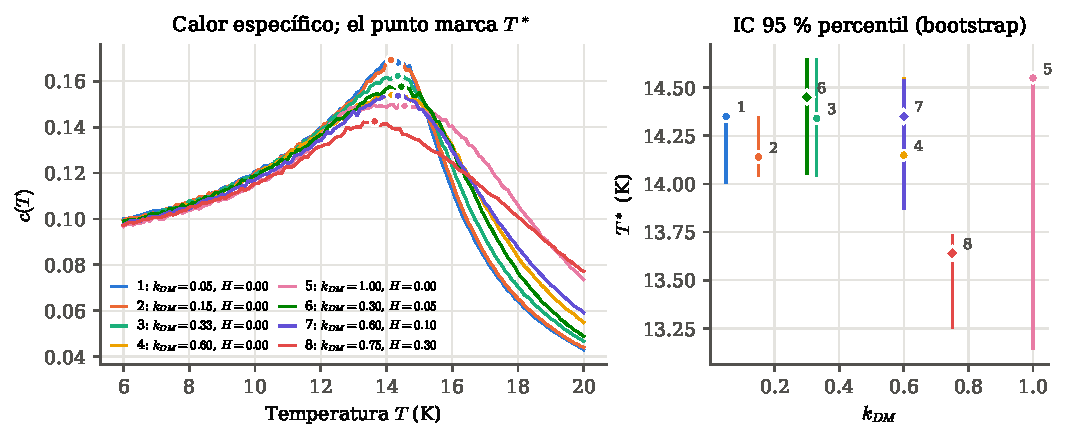
\includegraphics[width=\textwidth]{calor_especifico.pdf}
\caption{Izquierda: calor específico $c(T)$ de los ocho estados, promedio sobre 100 copias; el punto marca $T^*$. Derecha: $T^*$ frente a $\kdm$ con su intervalo percentil del 95~\%; círculos, $\Hex=0$; rombos, $\Hex>0$.}
\label{fig:calor}
\end{figure}

\begin{table}[H]
\centering\small
\caption{Temperatura del máximo de $c$. Bootstrap entre copias con $B=50\,000$. La meseta es el intervalo contiguo de la rejilla fina donde $c\ge c(T^*)-\widehat{\mathrm{se}}$, con $\widehat{\mathrm{se}}$ el error bootstrap de la altura del pico.}
\label{tab:tstar}
\begin{tabular}{ccccccc}
\toprule
Estado & $T^*$ (K) & se (K) & IC 95~\% percentil & IC 95~\% BCa & Meseta (K) & $c(T^*)$\\
\midrule
1 & 14.35 & 0.117 & [14.00, 14.37] & [14.14, 14.45] & [14.35, 14.40] & 0.170\\
2 & 14.14 & 0.068 & [14.04, 14.35] & [13.95, 14.14] & [14.11, 14.14] & 0.170\\
3 & 14.34 & 0.164 & [14.04, 14.65] & [13.85, 14.55] & [14.25, 14.34] & 0.163\\
4 & 14.15 & 0.127 & [14.04, 14.55] & [13.64, 14.15] & [14.15, 14.24] & 0.155\\
5 & 14.55 & 0.445 & [13.14, 14.55] & [13.55, 14.65] & [14.55, 14.58] & 0.151\\
6 & 14.45 & 0.166 & [14.05, 14.65] & [14.05, 14.65] & [14.45, 14.49] & 0.158\\
7 & 14.35 & 0.201 & [13.87, 14.54] & [13.94, 14.55] & [14.35, 14.44] & 0.155\\
8 & 13.64 & 0.127 & [13.25, 13.74] & [13.14, 13.64] & [13.60, 13.64] & 0.143\\
\bottomrule
\end{tabular}
\end{table}

En los ocho estados, $c(T)$ tiene un máximo ancho cerca de 14.3~K (figura~\ref{fig:calor} y tabla~\ref{tab:tstar}). Como verificación independiente, el argumento del máximo recalculado directamente sobre las varianzas de cada temperatura de la malla, sin repesado, cae a menos de 0.05~K del $T^*$ de la tabla en los ocho estados. Las diferencias entre estados se contrastaron con la diferencia bootstrap $T^{*b}(a)-T^{*b}(b)$ entre réplicas independientes y valores $p$ corregidos por Holm sobre los 28 pares \citep{holm1979}. Solo el estado 8, el de campo más intenso ($\Hex=0.3$), difiere: su $T^*$ es entre 0.5 y 0.8~K menor que el de los estados 1, 2, 3, 4 y 6 ($p$ ajustados de 0.002 a 0.037). Ningún otro par difiere. La correlación de Spearman entre $\kdm$ y $T^*$ es $\rho=0.05$ (prueba de permutación exacta sobre las $8!$ asignaciones, $p=0.90$): no se detecta una asociación monotónica en las ocho combinaciones. Este resultado no prueba independencia ni equivalencia de temperaturas.

Esta temperatura tiene una referencia física. Para el modelo de Heisenberg clásico en la red cúbica infinita, la transición ocurre en $k_BT_C=1.443\,J$ \citep{chen1993}, es decir $T_C\approx16.7$~K con $J=1$. El máximo observado cerca de 14.3~K es aproximadamente un 15~\% menor que esa referencia. Los bordes y el espesor pueden contribuir; la comparación cambia también anisotropía, interacción quiral y campo, de modo que no identifica un efecto exclusivo de tamaño. La susceptibilidad $\chi$ crece de forma monótona al enfriar y su máximo cae en el borde inferior de la escalera (de 6.0 a 8.4~K), de manera que no define $T^*$; además, depende de $m$, cuya convergencia es la más débil.

El intervalo del estado 5 ($\kdm=1$) es mucho más ancho que los demás, [13.14, 14.55]~K, porque su curva $c(T)$ tiene una cima casi plana entre 12.8 y 14.8~K (figura~\ref{fig:calor}). Sobre una cima plana, pequeñas fluctuaciones desplazan el argumento del máximo de un extremo a otro; la distribución bootstrap de $T^*$ resulta multimodal, con masas en 13.55, 14.05, 14.35 y 14.55~K. La inestabilidad corresponde al argmax sobre una región con máximos competitivos; requiere revisar la forma de la curva y las ranuras del repesado, y no permite diagnosticar por sí sola un error de simulación.

\section{Fase C: convergencia dentro de cada camino y entre caminos}
\label{sec:convergencia}

\subsection{Dos preguntas distintas}

Una cadena de Metropolis converge cuando la distribución de su estado ya no depende del punto de partida. Con 100 caminos independientes, esa propiedad se examina de dos maneras complementarias. Dentro de un camino, la serie medida debe ser estacionaria: su media no debe derivar entre el comienzo y el final de la medición. Entre caminos, todas las copias deben describir la misma distribución, porque todas parten de configuraciones distintas pero apuntan a la misma $\pi_\beta$. Una serie puede mostrar estabilidad local mientras permanece en un sector de energía. La comparación entre caminos puede detectar esa limitación si distintas copias ocupan sectores diferentes.

\textbf{Dentro de cada camino} se usaron tres herramientas. La prueba de \citet{geweke1992} compara la media del primer 10~\% de la serie con la del último 50~\% mediante $z=(\bar x_A-\bar x_B)/(\hat\sigma_A^2/n_A+\hat\sigma_B^2/n_B)^{1/2}$, con varianzas espectrales $\hat\sigma^2=\tauint s^2$. En cada temperatura se cuenta la proporción de copias con $|z|>1.96$ y se contrasta con el 5~\% nominal por una prueba binomial, con corrección de Holm sobre las temperaturas. El truncamiento MSER-5 de \citet{white1997} estima cuántos barridos iniciales siguen contaminados por el transitorio. El tiempo $\tauint$ y el tamaño efectivo $n_{\mathrm{ef}}$ completan el diagnóstico.

\textbf{Entre caminos}, la herramienta central es el factor de reducción de escala de \citet{gelman1992}. Con $m=100$ caminos de $n$ barridos, medias $\bar x_j$ y varianzas internas $s_j^2$,
\begin{equation}
W=\frac1m\sum_{j=1}^m s_j^2,\qquad
\frac{B}{n}=\frac{1}{m-1}\sum_{j=1}^m(\bar x_j-\bar x)^2,\qquad
\Rhat=\sqrt{\frac{\frac{n-1}{n}W+\frac{B}{n}}{W}} .
\label{eq:rhat}
\end{equation}
$W$ mide la variabilidad dentro de los caminos y $B/n$ la variabilidad de sus medias. Si todos los caminos muestrean la misma distribución, $B/n\approx\tauint W/n$ y $\Rhat\to1$ cuando $n$ crece. Si los caminos se quedan en valles distintos, $B/n$ no decrece y $\Rhat$ se estanca por encima de uno. El umbral usual es $\Rhat<1.01$ \citep{vehtari2021}. El veredicto oficial usó la versión normalizada por rangos y plegada de \citet{vehtari2021}, la más exigente; las figuras usan la forma clásica de la ecuación~(\ref{eq:rhat}), que permite separar $E$ de $m$. Se añadió una prueba $\chi^2$ de homogeneidad de las medias de las 100 copias, también con corrección de Holm.

Con estas herramientas, una temperatura \emph{converge} si cumple $\Rhat<1.01$ para $E$ y $m$, no presenta exceso de rechazos de Geweke y su truncamiento MSER-5 no supera 500 barridos. Es \emph{representativa} si además las copias son homogéneas. El criterio denominado \emph{confiable} exige por separado ESS mayor que 400 y jackknife por bloques admisible; no exige cumplir el criterio de convergencia. Esa independencia explica porcentajes de confiabilidad superiores a los de convergencia. Un estado converge solo si todas sus 141 temperaturas lo hacen.

\begin{table}[H]
\centering\small
\caption{Veredicto oficial: porcentaje de las 141 temperaturas que cumplen cada criterio y tramo continuo desde 20~K. Ningún estado converge en toda la escalera.}
\label{tab:veredicto}
\begin{tabular}{lcccccccc}
\toprule
Estado & 1 & 2 & 3 & 4 & 5 & 6 & 7 & 8\\
\midrule
Converge (\%) & 30 & 31 & 38 & 54 & 55 & 30 & 38 & 40\\
Tramo convergido (K) & 15.9 & 15.7 & 14.7 & 13.8 & 13.7 & 15.8 & 15.1 & 14.7\\
Representativa (\%) & 29 & 31 & 38 & 46 & 38 & 28 & 36 & 40\\
Confiable (\%) & 30 & 31 & 38 & 72 & 100 & 32 & 40 & 41\\
\bottomrule
\end{tabular}
\end{table}

La tabla~\ref{tab:veredicto} es concluyente en lo global: ningún estado converge en toda la escalera. El mejor caso, $\kdm=1$, cumple en el 55~\% de las temperaturas, sin interrupción de 20.0 a 13.7~K. Por debajo de ese tramo, los resultados no pueden tomarse como muestras de la distribución de equilibrio.

\subsection{Qué converge y qué no: energía frente a magnetización}

La figura~\ref{fig:rhat} separa el diagnóstico por variable y aclara el veredicto. Para la energía, $\Rhat-1$ queda por debajo de 0.01 en todas las temperaturas de siete estados y en el 93~\% de las del estado 5, con un máximo de 1.017. La magnetización se comporta distinto: $\Rhat$ sube de forma sostenida al enfriar, cruza el umbral entre 15.5 y 9.5~K según el estado y alcanza 2.8 a 6~K. El veredicto negativo se debe a $m$, no a $E$.

\begin{figure}[H]
\centering
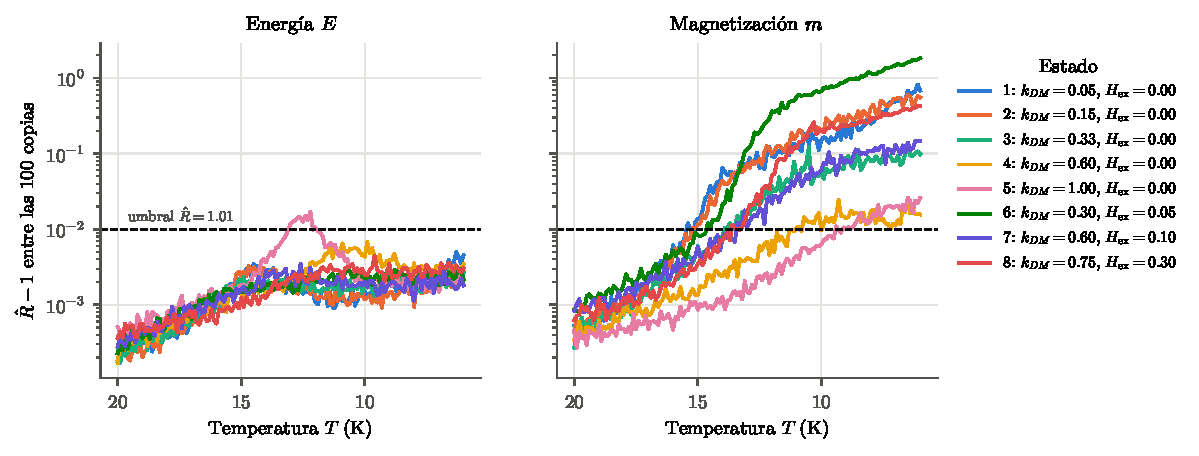
\includegraphics[width=0.92\textwidth]{rhat_T.pdf}
\caption{$\Rhat-1$ entre las 100 copias en cada temperatura, en escala logarítmica. La línea discontinua es el umbral $\Rhat=1.01$; el eje de temperatura avanza en el sentido del enfriamiento.}
\label{fig:rhat}
\end{figure}

\begin{figure}[H]
\centering
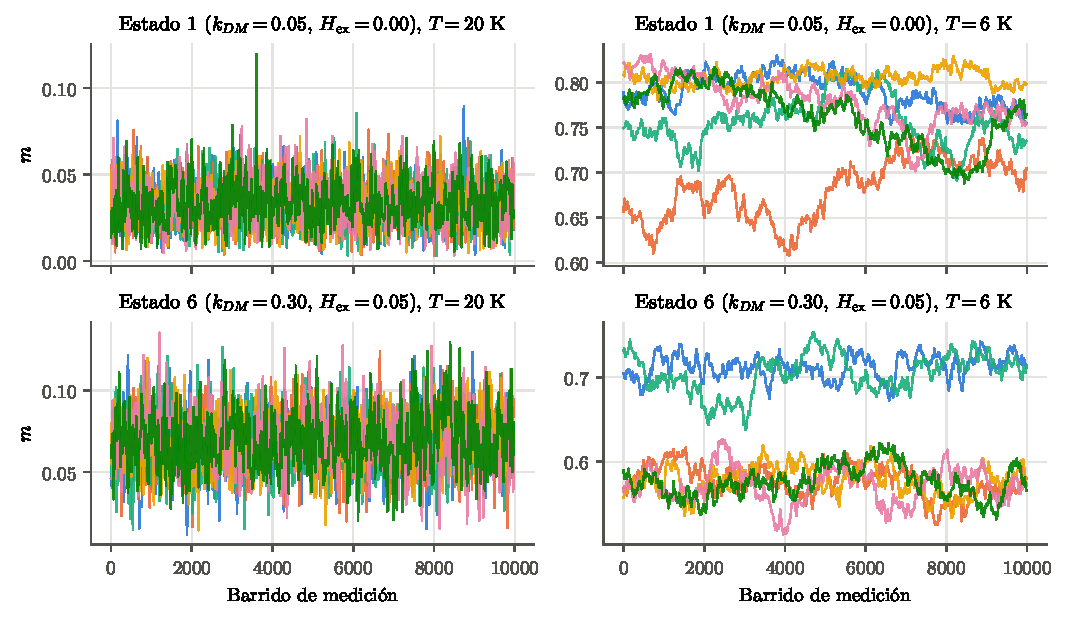
\includegraphics[width=0.88\textwidth]{trazas_m.pdf}
\caption{Magnetización de seis copias durante los 10\,000 barridos de medición (una muestra cada 20 barridos). A 20~K los caminos son indistinguibles; a 6~K cada camino es estable alrededor de su propio nivel y los niveles difieren entre caminos.}
\label{fig:trazas}
\end{figure}

La figura~\ref{fig:trazas} muestra el mecanismo. A 20~K las seis trayectorias se superponen: no se observan diferencias persistentes en esas trazas, de acuerdo con los diagnósticos a esa temperatura. A 6~K cada trayectoria es aproximadamente estacionaria, de modo que el diagnóstico dentro del camino es favorable, pero cada una oscila alrededor de un nivel distinto. En el estado 6 las copias se separan en dos grupos, cerca de $m=0.58$ y $m=0.70$. Así se resuelve la aparente paradoja: dentro de un mismo camino la medición se mantiene igual, como debe ocurrir; entre caminos, la orientación de la textura difiere. Las diferencias de $m$ requieren cambios de alineación relativa, cancelación entre dominios o textura: una rotación rígida conserva la norma de magnetización. Configuraciones con distinta $m$ pueden tener energías próximas. Esa posibilidad explica la diferencia entre diagnósticos, pero la estabilidad de $E$ sola no garantiza la de su varianza. La auditoría adicional examina la fluctuación energética cuadrática cerca del pico.

\subsection{Cuántos pasos Monte Carlo hacen falta}

La pregunta práctica es cuántos barridos adicionales llevarían a $\Rhat<1.01$. Para responderla se recalculó $\Rhat$ con los primeros $n$ barridos de medición, para 25 valores de $n$ entre 100 y 10\,000 (figura~\ref{fig:rhatn}). Si los caminos exploran la misma distribución, $B/n$ decae como $1/n$ y la pendiente de $\log(\Rhat-1)$ frente a $\log n$ es cercana a $-1$. Una pendiente mucho menor en valor absoluto indica caminos atrapados.

\begin{figure}[H]
\centering
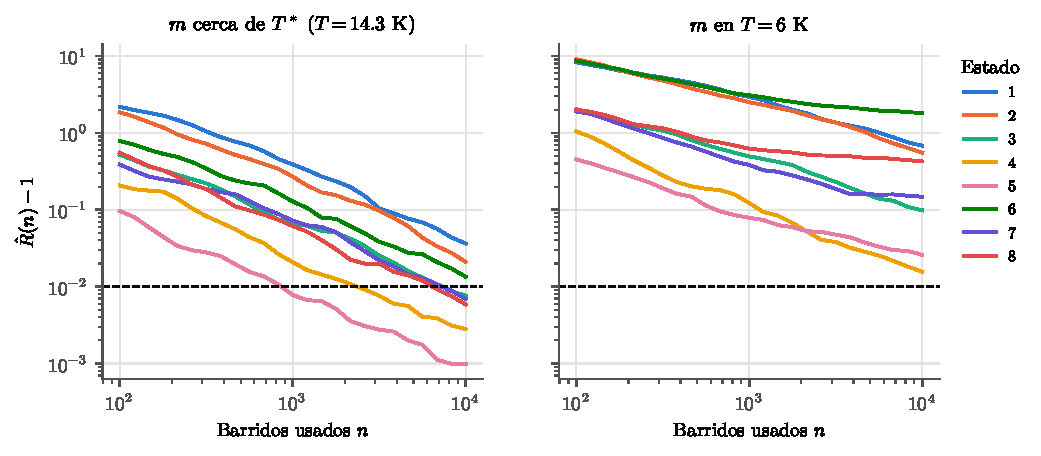
\includegraphics[width=0.88\textwidth]{rhat_n.pdf}
\caption{$\Rhat(n)-1$ de la magnetización calculado con los primeros $n$ barridos de medición, cerca de $T^*$ (izquierda) y a 6~K (derecha). La línea discontinua es el umbral.}
\label{fig:rhatn}
\end{figure}

\begin{figure}[H]
\centering
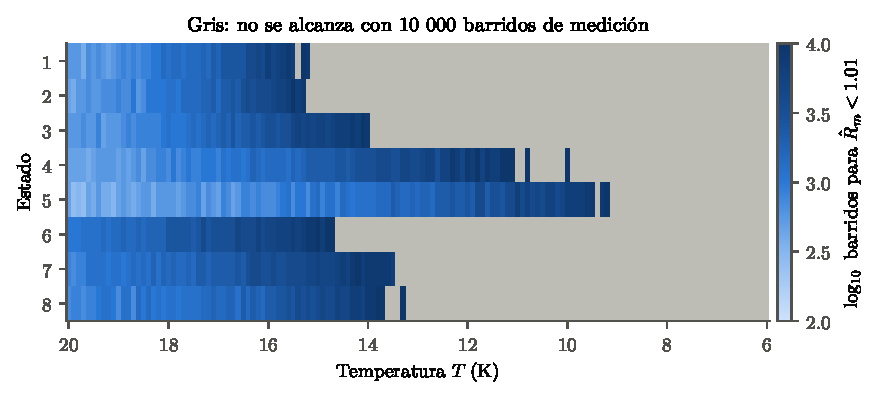
\includegraphics[width=0.92\textwidth]{barridos_necesarios.pdf}
\caption{Barridos de medición necesarios para que $\Rhat_m$ quede por debajo de 1.01 y no vuelva a superarlo, por estado y temperatura. En gris, temperaturas donde 10\,000 barridos no bastan.}
\label{fig:barridos}
\end{figure}

Cerca de $T^*$ la pendiente vale entre $-0.88$ y $-1.08$ en los ocho estados: el régimen es de mezcla lenta pero sana, y la extrapolación orienta hacia $10^4$ a $3.4\times10^4$ barridos. Es una proyección desde la ventana observada y necesita validación mediante corridas más largas. A 6~K aparecen dos comportamientos. En los estados sin campo, la pendiente se mantiene entre $-0.48$ y $-0.87$, y la extrapolación da $1.6\times10^4$ barridos para $\kdm=0.6$, $2.1\times10^5$ para $\kdm=0.33$ y de $4\times10^6$ a $8\times10^6$ para $\kdm\le0.15$, es decir, de 400 a 800 veces el presupuesto usado. Con campo, la pendiente se aplana: $-0.43$ en el estado 7, que necesitaría $3.5\times10^6$ barridos, y $-0.22$ y $-0.15$ en los estados 6 y 8. En estos dos últimos, $\Rhat$ prácticamente no baja con más barridos, y la extrapolación supera los $10^{13}$, una cifra sin utilidad predictiva a esa distancia de los datos. La pendiente observada advierte que debe compararse otro esquema de muestreo antes de invertir en cadenas mucho más largas. La figura~\ref{fig:barridos} resume el mapa completo; el límite entre azul y gris es la temperatura a la que el presupuesto se agotó.

\subsection{Relación con la interacción quiral y el campo}

\begin{table}[H]
\centering\small
\caption{Correlación de Spearman entre los parámetros y las métricas de convergencia de $m$, sobre los ocho estados. IC bootstrap percentil del 95~\% remuestreando estados ($B=20\,000$) y valor $p$ de la prueba de permutación exacta ($8!=40\,320$ asignaciones).}
\label{tab:spearman}
\begin{tabular}{llccc}
\toprule
Métrica & Parámetro & $\rho$ & IC 95~\% & $p$\\
\midrule
fracción de T con $\hat R_m<1.01$ & $k_{DM}$ & $+0.92$ & $[+0.47,\,+1.00]$ & 0.003 \\
fracción de T con $\hat R_m<1.01$ & $H$ & $+0.11$ & $[-0.60,\,+0.84]$ & 0.801 \\
T más baja del tramo convergido en $m$ (K) & $k_{DM}$ & $-0.92$ & $[-1.00,\,-0.47]$ & 0.002 \\
T más baja del tramo convergido en $m$ (K) & $H$ & $-0.11$ & $[-0.81,\,+0.59]$ & 0.827 \\
$\tau_{int}$ máximo de $m$ (barridos) & $k_{DM}$ & $-0.96$ & $[-1.00,\,-0.64]$ & 0.001 \\
$\tau_{int}$ máximo de $m$ (barridos) & $H$ & $-0.14$ & $[-0.94,\,+0.55]$ & 0.762 \\
$\tau_{int}$ máximo de $E$ (barridos) & $k_{DM}$ & $-0.20$ & $[-1.00,\,+0.65]$ & 0.631 \\
$\tau_{int}$ máximo de $E$ (barridos) & $H$ & $-0.52$ & $[-0.96,\,+0.18]$ & 0.208 \\
\bottomrule
\end{tabular}
\end{table}

\begin{figure}[H]
\centering
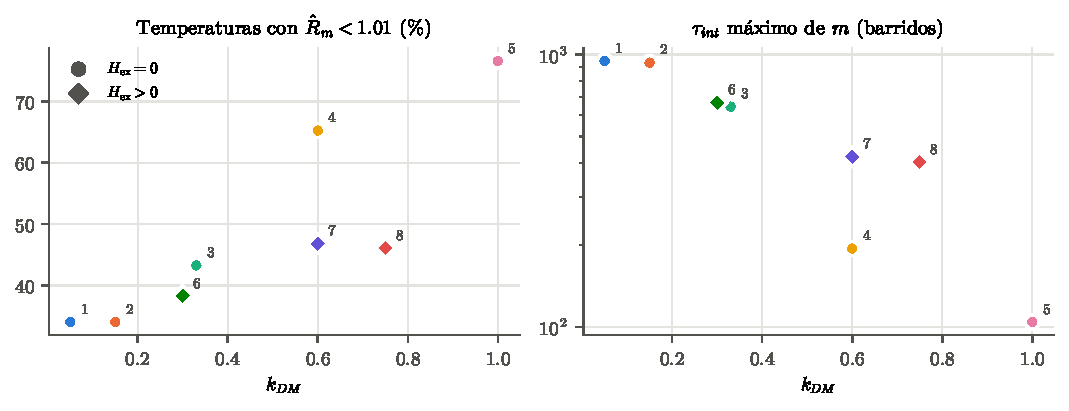
\includegraphics[width=0.9\textwidth]{correlacion_kdm.pdf}
\caption{Fracción de temperaturas convergidas en $m$ (izquierda) y $\tauint$ máximo de $m$ (derecha) frente a $\kdm$. Círculos: $H=0$; rombos: $H>0$; el número identifica el estado.}
\label{fig:corr}
\end{figure}

La interacción quiral gobierna el costo de convergencia de la magnetización (tabla~\ref{tab:spearman} y figura~\ref{fig:corr}). Al pasar de $\kdm=0.05$ a $\kdm=1$, el $\tauint$ máximo de $m$ baja de 946 a 104 barridos ($\rho=-0.96$, $p=0.001$), la fracción de temperaturas convergidas sube del 34 al 77~\% ($\rho=0.92$, $p=0.003$) y el tramo convergido se extiende de 15.5 a 9.5~K. Para la energía no hay relación ($\rho=-0.20$, $p=0.63$). Con solo ocho estados, los intervalos son anchos y la correlación marginal con $H$ no es significativa; además, $H$ y $\kdm$ están confundidos en el diseño, pues los tres estados con campo tienen $\kdm$ intermedio o alto.

Para describir asociaciones condicionadas a ambos parámetros se ajustó por mínimos cuadrados, sobre los $8\times141$ pares (estado, temperatura),
\begin{equation}
\log\tauint(m)=\underset{(0.10)}{3.03}-\underset{(0.07)}{2.37}\,\kdm+\underset{(0.22)}{2.75}\,H+\underset{(0.79)}{30.6}\,\frac1T,\qquad R^2=0.70,
\label{eq:regresion}
\end{equation}
con errores estándar de tipo sándwich (HC0), válidos bajo heterocedasticidad, entre paréntesis. A temperatura fija, aumentar $\kdm$ en 0.1 reduce $\tauint$ en un 21~\% ($e^{-0.237}$), mientras que aumentar $H$ en 0.1 lo multiplica por 1.32. Enfriar de 20 a 6~K lo multiplica por $e^{30.6(1/6-1/20)}\approx35$. Los pares con igual $\kdm$ confirman el signo del campo: con $\kdm=0.6$, $\tauint$ pasa de 194 barridos ($H=0$) a 421 ($H=0.1$). Los errores estándar de la ecuación~(\ref{eq:regresion}) son optimistas, porque temperaturas vecinas de un mismo estado no son independientes; la inferencia sobre los parámetros descansa en la prueba de permutación entre estados. La misma regresión para la energía explica apenas el 24~\% de la variación, con un coeficiente de $\kdm$ de 0.29.

La escala espacial ofrece una explicación plausible para el signo observado de $\kdm$. La espiral tiene período $\lambda=2\pi/\arctan(\kdm/J)$, y el factor de estructura de las configuraciones finales lo confirma: con $\kdm$ de 0.33, 0.6 y 1.0 se miden 18.1, 10.1 y 7.0 sitios, frente a 19.7, 11.6 y 8.0 de la fórmula. Con $\kdm\le0.15$ el período teórico supera los 42 sitios, más que el diámetro del disco (37 sitios), y el período medido se satura en 30.2. Cuando la espiral no cabe en el disco, la textura es casi un único dominio con magnetización neta grande, y su orientación solo cambia rotando el disco entero, un movimiento colectivo que Metropolis, espín por espín, ejecuta con extrema lentitud. Con $\kdm$ grande caben varias vueltas de espiral, la magnetización se promedia entre dominios y cada camino la decorrelaciona pronto. El campo perpendicular, por su parte, estabiliza skyrmiones: a 6~K la carga topológica modal es $Q=0$ en los estados sin campo y $Q=-1$, $-4$ y $-6$ en los estados 6, 7 y 8. Cambiar la categoría de $Q$ puede requerir reorganizaciones difíciles con movimientos locales. Las configuraciones finales y el estancamiento del diagnóstico son compatibles con mezcla limitada, pero no se guardó la trayectoria de $Q$ por barrido para medir tasas de cambio de sector o demostrar que nunca ocurre.

\subsection{Poblaciones ocultas de estados finales: mezclas y algoritmo EM}

Si los caminos terminan en valles distintos, las medias $\bar m_j$ de las 100 copias a 6~K deben provenir de una mezcla de poblaciones. Se ajustaron mezclas gaussianas de $k=1$, 2 y 3 componentes con el algoritmo EM \citep{dempster1977}, programado sin librerías de mezclas. El paso E calcula las responsabilidades $r_{jc}=w_c\,\phi(\bar m_j;\mu_c,\sigma_c^2)/\sum_\ell w_\ell\,\phi(\bar m_j;\mu_\ell,\sigma_\ell^2)$; el paso M actualiza $w_c=\sum_jr_{jc}/100$, $\mu_c$ y $\sigma_c^2$ como medias y varianzas ponderadas. Para cada $k$ se usaron 20 arranques aleatorios, se conservó el de mayor verosimilitud y se eligió $k$ con $\mathrm{BIC}=-2\ell+(3k-1)\log100$ \citep{schwarz1978}. En los 480 ajustes la log-verosimilitud nunca decreció entre iteraciones, como garantiza la teoría del algoritmo.

\begin{table}[H]
\centering\small
\caption{Mezclas gaussianas ajustadas por EM a las medias $\bar m_j$ de las 100 copias a 6~K. Se elige el $k$ de menor BIC; la última columna muestra los pesos y las componentes del modelo elegido.}
\label{tab:em}
\footnotesize\setlength{\tabcolsep}{4pt}
\begin{tabular}{cccccp{8.2cm}}
\toprule
Estado & BIC $k=1$ & BIC $k=2$ & BIC $k=3$ & $k$ & Componentes\\
\midrule
1 & -380.4 & -411.8 & -405.2 & 2 & 0.72\,$\mathcal N(0.775,\,0.015^2)$; 0.28\,$\mathcal N(0.714,\,0.033^2)$ \\
2 & -290.0 & -280.5 & -271.4 & 1 & 1.00\,$\mathcal N(0.300,\,0.054^2)$ \\
3 & -634.0 & -622.9 & -611.5 & 1 & 1.00\,$\mathcal N(0.065,\,0.010^2)$ \\
4 & -959.6 & -948.9 & -943.6 & 1 & 1.00\,$\mathcal N(0.027,\,0.002^2)$ \\
5 & -1004.8 & -1014.8 & -1011.0 & 2 & 0.60\,$\mathcal N(0.015,\,0.001^2)$; 0.40\,$\mathcal N(0.017,\,0.001^2)$ \\
6 & -300.9 & -589.3 & -582.6 & 2 & 0.78\,$\mathcal N(0.580,\,0.007^2)$; 0.22\,$\mathcal N(0.702,\,0.006^2)$ \\
7 & -675.3 & -726.1 & -718.8 & 2 & 0.82\,$\mathcal N(0.389,\,0.003^2)$; 0.18\,$\mathcal N(0.372,\,0.008^2)$ \\
8 & -619.1 & -669.3 & -720.9 & 3 & 0.50\,$\mathcal N(0.577,\,0.003^2)$; 0.39\,$\mathcal N(0.563,\,0.002^2)$; 0.11\,$\mathcal N(0.595,\,0.002^2)$ \\
\bottomrule
\end{tabular}
\end{table}

\begin{figure}[H]
\centering
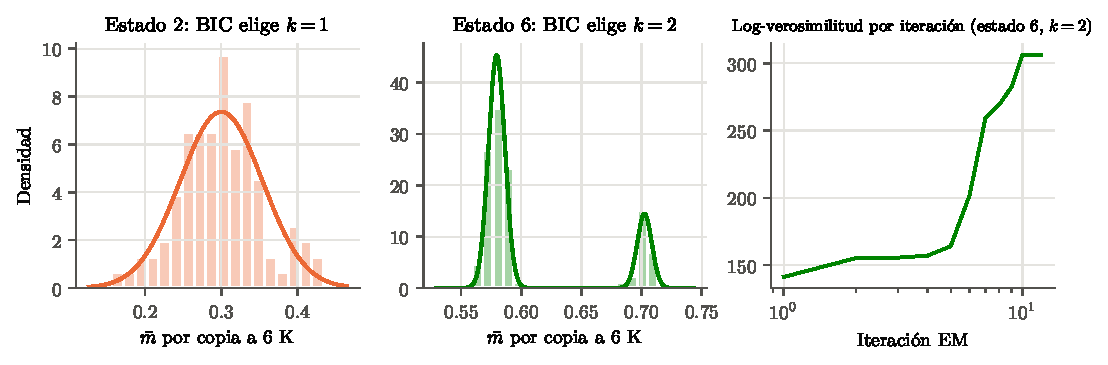
\includegraphics[width=0.95\textwidth]{mezcla_em.pdf}
\caption{Histograma de $\bar m_j$ a 6~K con la mezcla elegida por BIC para los estados 2 y 6, y log-verosimilitud por iteración del mejor arranque del estado 6 con $k=2$.}
\label{fig:em}
\end{figure}

El BIC distingue dos situaciones (tabla~\ref{tab:em} y figura~\ref{fig:em}). En los estados 2, 3 y 4 basta una normal: una sola población estadística describe las medias de $m$ entre las opciones probadas; ello no identifica un único valle físico. En los estados 1, 6 y 8 hay poblaciones separadas. El caso más nítido es el estado 6: el 78~\% de los caminos termina cerca de $m=0.58$ y el 22~\% cerca de $m=0.70$, con desviaciones internas de 0.007, de modo que los grupos no se solapan. La proporción dominante coincide con la del agrupamiento jerárquico del factor de estructura (78~\%). Esa igualdad apoya una comparación entre clasificaciones, pero no demuestra correspondencia individual sin cruzar las etiquetas de cada camino. En el estado 8 el BIC elige tres componentes y la mitad de los caminos comparte la carga modal $Q=-6$. En los estados 5 y 7 las componentes tienen casi la misma media y difieren sobre todo en dispersión; allí la mezcla describe diferencias estadísticas entre caminos y no basta para identificar valles físicos distintos. Estas poblaciones describen la diversidad del protocolo finito. Las realizaciones son válidas para ese protocolo y algunas ventanas pasan pruebas locales de estabilidad; ello no demuestra estacionariedad global ni pesos de Boltzmann. Los pesos de la mezcla son frecuencias de llegada y sus componentes no equivalen automáticamente a fases termodinámicas.

\section{Auditoría adicional de los datos y utilidad del protocolo}
\label{sec:auditoria}

\subsection{Estabilidad de los momentos de energía}

El calor específico depende de $\langle E^2\rangle-\langle E\rangle^2$, de modo que un diagnóstico favorable solo para $E$ no basta. La auditoría local calculó el máximo del $\hat R$ dividido, normalizado por rangos y plegado para $E$, $(E-\bar E)^2$ y $m$. El centro $\bar E$ es común a las 100 copias de una temperatura. Se revisaron siete puntos por estado: 6, 10 y 20~K y cuatro temperaturas medidas alrededor de su $T^*$. Son 56 puntos; no se afirma haber repetido esta prueba en toda la escalera.

\begin{table}[H]\centering\small
\caption{Máximo del diagnóstico entre los cuatro puntos medidos próximos a $T^*$ en cada estado. La fluctuación cuadrática energética muestra mayor estabilidad entre caminos que la magnetización.}
\begin{tabular}{ccc}\toprule Estado & $\hat R$ de $(E-\bar E)^2$ & $\hat R$ de $m$\\\midrule
1 & 1.001139 & 1.084110 \\
2 & 1.001005 & 1.074655 \\
3 & 1.000891 & 1.014063 \\
4 & 1.000895 & 1.005463 \\
5 & 1.000928 & 1.002185 \\
6 & 1.000753 & 1.026242 \\
7 & 1.000808 & 1.014595 \\
8 & 1.000772 & 1.021573 \\
\bottomrule\end{tabular}\end{table}

Los 32 puntos próximos al máximo cumplen $\hat R<1.002$ para la fluctuación cuadrática. Esto refuerza la evidencia sobre los momentos observados de energía. Los sectores que ninguno de los caminos haya visitado siguen fuera del alcance del diagnóstico. Por ello se conserva una interpretación condicionada de la estimación termodinámica.

\subsection{Regresión con temperaturas agrupadas y sensibilidad}

El ajuste sobre 1128 pares reproduce los coeficientes originales. La revisión calcula una covarianza sándwich agrupada en los ocho estados, con corrección CR1, y repite el ajuste omitiendo un estado cada vez. Los errores HC0 no corrigen la dependencia de temperaturas de un mismo camino.

\begin{table}[H]\centering\small
\caption{Sensibilidad de la regresión. Los errores agrupados aumentan y el coeficiente del campo depende de una combinación influyente. Con ocho grupos, la inferencia sigue siendo exploratoria.}
\begin{tabular}{lrrrr}\toprule Parámetro & Estimación & se HC0 & se CR1 & Rango al retirar un estado\\\midrule
Intercepto & 3.0291 & 0.0986 & 0.2009 & [2.9072, 3.1837] \\
$k_{DM}$ & -2.3653 & 0.0723 & 0.1450 & [-2.5773, -2.2520] \\
$H$ & 2.7487 & 0.2170 & 0.5366 & [2.3520, 6.1538] \\
$1/T$ & 30.6096 & 0.7916 & 2.0863 & [29.4760, 31.4989] \\
\bottomrule\end{tabular}\end{table}

Al omitir el estado 8, el coeficiente de $H$ pasa de 2.749 a 6.154. El signo del coeficiente de $\kdm$ se mantiene en los ocho ajustes. Estas pruebas evalúan sensibilidad y no sustituyen un diseño factorial. La permutación exacta de la asociación entre $\kdm$ y $T^*$ se reprodujo con $\rho=0.0542169$ y $p=0.899256$; no rechazar asociación nula no demuestra equivalencia.

\subsection{Fluctuaciones del protocolo y evolución de los ocho estados}

La revisión leyó la magnetización de los 1128 archivos, cada uno con $10000\times100$ mediciones. Calculó la media del protocolo, su error entre caminos, los percentiles 10 y 90 de las medias por copia y la contribución entre caminos a la varianza. Con divisores poblacionales y cadenas de igual longitud,
\begin{equation}
\widehat{\operatorname{Var}}(m)=\frac1R\sum_j\widehat{\operatorname{Var}}_t(m_j)+\frac1R\sum_j(\bar m_j-\bar m)^2.
\end{equation}
La segunda contribución mide diferencias persistentes entre historias. Si sus frecuencias no son pesos de Boltzmann, $N\operatorname{Var}(m)/(k_BT)$ describe fluctuaciones del protocolo y no una susceptibilidad de equilibrio demostrada. Además, la respuesta al campo $H$ involucra la componente $M_z$ conjugada a él, no automáticamente la norma $m$.

\begin{figure}[H]\centering
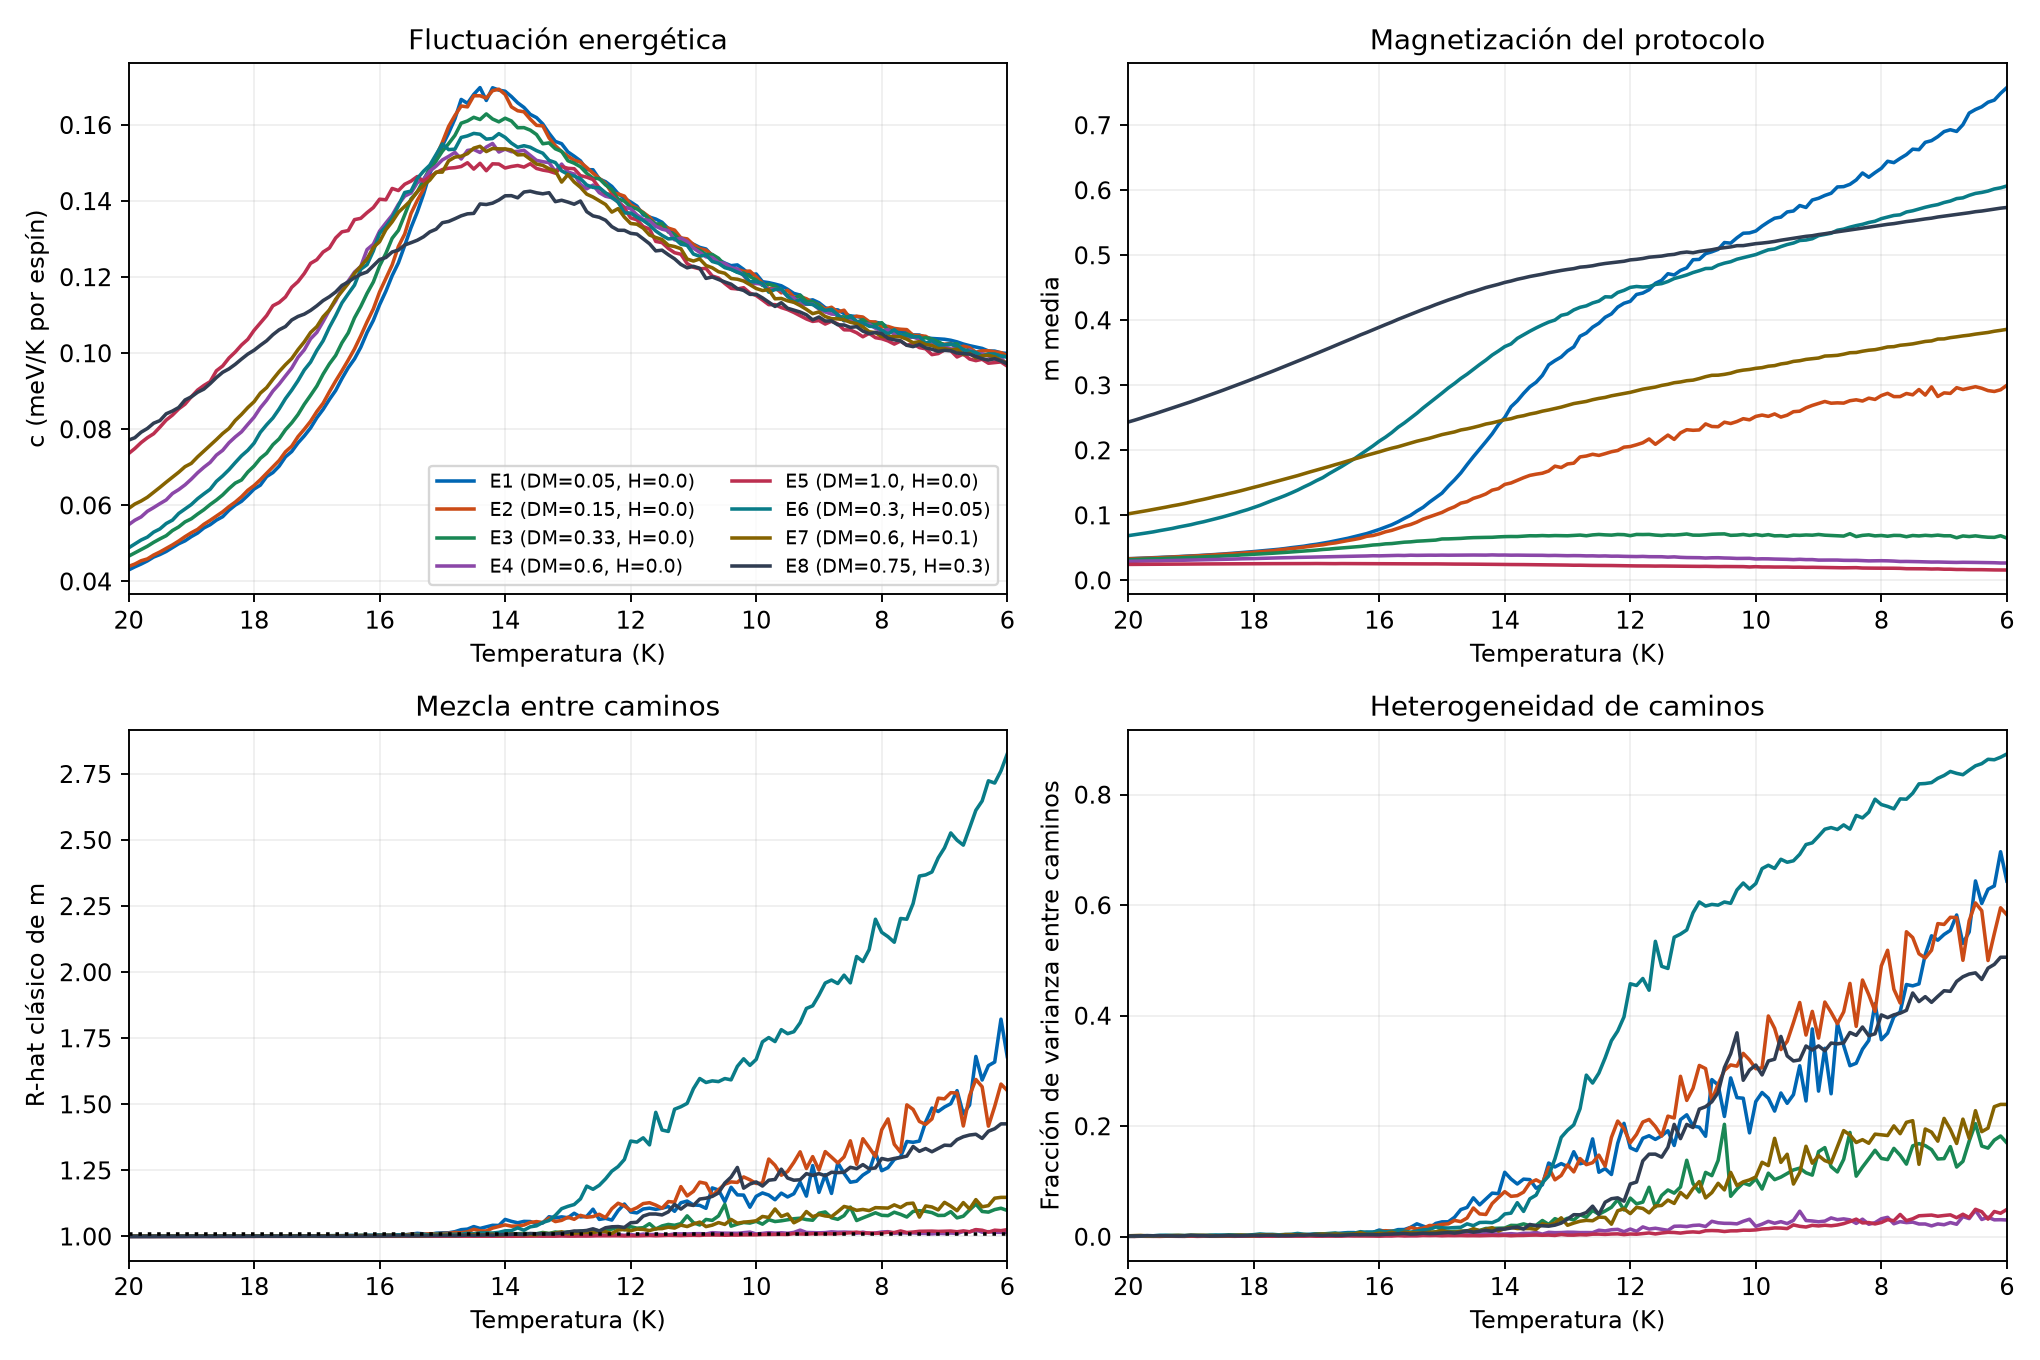
\includegraphics[width=\textwidth]{fig/comparacion_ocho_estados.png}
\caption{Curvas de los ocho estados en las 141 temperaturas: fluctuación energética, magnetización del protocolo, diagnóstico clásico de mezcla y fracción de varianza de $m$ entre caminos.}
\label{fig:ochoestados}
\end{figure}

Las configuraciones de las primeras tres copias, en 16 temperaturas y en la capa central, se incorporaron al explorador HTML. Son instantáneas finales por temperatura y permiten seguir caminos fijos. Las frecuencias de texturas se estudian con las 100 copias, no con esos tres ejemplos. Con bordes libres, la carga geométrica puede no ser entera; las categorías modales originales redondean el promedio entre capas. No se registró $Q$ a cada barrido, así que no se midieron tasas de transición entre categorías.

\section{Discusión, conclusiones y transparencia}

\subsection{Respuesta a las preguntas del proyecto}

El máximo de la fluctuación energética identifica una temperatura característica cercana a 14.3~K en siete estados y de 13.64~K en el estado 8. Es una escala pseudocrítica del disco finito y del ensamble observado. El tamaño del sistema y la presencia de campo impiden identificarla automáticamente con una singularidad de Curie. La auditoría de los momentos energéticos cerca del máximo aporta evidencia favorable para esa estimación, sin demostrar mezcla global.

No se detecta asociación monotónica entre $\kdm$ y $T^*$ ($\rho=0.05$, $p=0.90$). La ausencia de rechazo no establece independencia ni equivalencia. El estado 8 difiere de cinco combinaciones bajo las comparaciones bootstrap corregidas, pero cambia a la vez campo e interacción quiral. El diseño no atribuye todo el desplazamiento al campo.

Ningún estado pasa el criterio conjunto de convergencia en toda la escalera. La magnetización conserva diferencias entre caminos al enfriar, mientras que los momentos energéticos examinados cerca del pico muestran mayor estabilidad. Los caminos son realizaciones válidas del enfriamiento; sus proporciones finales describen el protocolo y no son pesos de equilibrio demostrados.

\subsection{Resultados útiles para estudiar las texturas}

La asociación de $\kdm$ con el costo de decorrelación de $m$ conserva el signo al retirar cualquiera de los estados. Los períodos espaciales y la cancelación entre dominios ofrecen una interpretación física de ese comportamiento. Una rotación rígida no cambia $m$; las diferencias entre caminos requieren variación de la textura o de la alineación relativa.

El par de estados 4 y 7 mantiene $\kdm=0.6$ y permite comparar $H=0$ con $H=0.1$: el máximo observado de $\tauint(m)$ pasa de 194 a 421 barridos. Es una comparación puntual útil. La regresión general conserva el signo del campo, pero su magnitud es sensible al estado 8 y sus errores aumentan al agrupar por estado. Con solo ocho grupos, el ajuste tiene alcance exploratorio.

En el estado 6, las medias de magnetización a 6~K forman dos poblaciones bien separadas. En el estado 8, el BIC selecciona tres componentes. Esas poblaciones y las cargas finales permiten estudiar memoria del camino y diversidad de texturas, aun donde no se ha demostrado equilibrio. Las componentes gaussianas son una descripción estadística y deben contrastarse con clasificaciones espaciales por copia.

\subsection{Conclusiones}

\begin{enumerate}
\item Las curvas energéticas sitúan una temperatura característica alrededor de 14~K. La incertidumbre del argmax es especialmente grande en el estado 5 y exige conservar la distribución bootstrap completa.
\item La auditoría adicional de la fluctuación energética cuadrática pasa el umbral de $\hat R<1.002$ en los 32 puntos próximos a los máximos. Esta evidencia respalda los momentos observados usados en $c(T)$; no prueba exploración de todos los sectores.
\item La magnetización presenta mezcla limitada a baja temperatura. La descomposición de su varianza separa fluctuaciones internas y diferencias entre historias, y permite interpretar qué parte de la curva agrupada procede de heterogeneidad del protocolo.
\item Las relaciones con $\kdm$ y $H$ orientan nuevos experimentos, pero el diseño incompleto y sus ocho estados limitan la atribución causal. Las extrapolaciones a millones de barridos son señales de dificultad, no predicciones de costo verificadas.
\end{enumerate}

\subsection{Limitaciones y siguientes pruebas}

Un diseño factorial en $\kdm$ y $H$ permitiría separar sus asociaciones. Variar radio y espesor con el mismo hamiltoniano permitiría evaluar confinamiento. Cambiar duración del enfriamiento y comparar calentamiento permitiría medir dependencia del protocolo. Los barridos no son tiempo físico calibrado.

Para evaluar mezcla conviene registrar la termalización, guardar $Q$ y las componentes de magnetización durante la medición y comparar inicializaciones diferentes. El intercambio de réplicas y los movimientos colectivos son candidatos a estudiar; no se ejecutaron en esta revisión. Su evaluación requiere cambios de sector y viajes completos por la escalera, además de aceptación de intercambios.

\subsection{Transparencia y reproducibilidad}

El análisis original recibió apoyo del asistente Claude Code en depuración, programación y redacción, según la declaración previa del proyecto. La revisión local con Codex añadió pruebas de momentos en 56 puntos, covarianza agrupada por estado, sensibilidad al retirar estados, permutación exacta y curvas de magnetización en las 1128 combinaciones. No volvió a ejecutar la simulación ni el bootstrap de 50000 réplicas. Los programas, resultados derivados y registros se conservan en \texttt{scripts/auditoria/} y \texttt{resultados/auditoria/}; el desarrollo matemático y los exploradores se incluyen en \texttt{docs/explicacion\_completa.html}. La escritura sigue las pautas del marco Morfeo instalado.


\bibliographystyle{apalike}
\bibliography{refs}

\appendix
\section{Anexo: reproducibilidad}

\textbf{Simulación.} Cuadernos \texttt{simulacion/lotes/lote\_0X.ipynb} (JAX, dos GPU T4 en Kaggle, semilla fija por lote). Cada temperatura se guarda en el archivo\\ \texttt{lote\_0X/estado\_N/T\_<T>.npz}, con las series $E$, $m$ y componentes de energía ($10\,000\times100$), los espines finales, los parámetros físicos y las claves aleatorias; la escritura es atómica y verifica dimensiones, finitud y norma de los espines.

\textbf{Análisis oficial.} \texttt{scripts/analisis/dmi\_analisis.py} y \texttt{scripts/analisis/ejecutar.py}, ejecutados en CPU con 32 procesos y $B=50\,000$: diagnósticos por temperatura, jackknife, bootstrap, repesado, $T^*$, carga topológica y factor de estructura. Tablas en \texttt{resultados/}.

\textbf{Análisis de este informe.} Todos con semilla 20261117 y ejecutables de principio a fin sin intervención:
\begin{itemize}
\item \texttt{pasos\_mc.py}: $\Rhat$ clásico, $W$, $B/n$ y $\tauint$ por estado y temperatura, y $\Rhat(n)$ sobre 25 valores de $n$.
\item \texttt{figuras\_informe.py}: figuras~\ref{fig:rhat}, \ref{fig:trazas}, \ref{fig:rhatn}, \ref{fig:barridos} y \ref{fig:corr}, correlaciones de Spearman con permutación exacta y bootstrap, y la regresión de la ecuación~(\ref{eq:regresion}).
\item \texttt{figura\_calor.py}: figura~\ref{fig:calor} y la verificación independiente de $T^*$.
\item \texttt{mezcla\_em.py}: mezclas gaussianas por EM y selección por BIC (tabla~\ref{tab:em} y figura~\ref{fig:em}).
\item \texttt{uniformidad.py}: prueba $\chi^2$ del generador por transformada inversa con 100 semillas.
\end{itemize}

\textbf{Uso de librerías.} Los generadores no uniformes, el bootstrap, el jackknife, el EM, $\Rhat$, $\tauint$, la regresión y las correlaciones se programaron con operaciones básicas de NumPy. Se usaron funciones de librería solo para la transformada rápida de Fourier, el álgebra de matrices, las funciones especiales que dan valores $p$ ($\Gamma$ incompleta, normal estándar, binomial) y el agrupamiento jerárquico del factor de estructura.

\begin{table}[H]
\centering\small
\caption{Diagnósticos por variable con la convención $\tauint=1+2\sum\rho$. Fracción de temperaturas con $\Rhat<1.01$ y $\tauint$ máximo sobre la escalera.}
\begin{tabular}{lcccccccc}
\toprule
Estado & 1 & 2 & 3 & 4 & 5 & 6 & 7 & 8\\
\midrule
$\Rhat_E<1.01$ (\%) & 100 & 100 & 100 & 100 & 93 & 100 & 100 & 100\\
$\Rhat_m<1.01$ (\%) & 34 & 34 & 43 & 65 & 77 & 38 & 47 & 46\\
$\tauint$ máx de $E$ & 52 & 47 & 38 & 30 & 57 & 32 & 32 & 30\\
$\tauint$ máx de $m$ & 946 & 933 & 643 & 194 & 104 & 665 & 421 & 403\\
Tramo convergido en $m$ (K) & 15.5 & 15.3 & 14.0 & 11.1 & 9.5 & 14.7 & 13.5 & 13.7\\
\bottomrule
\end{tabular}
\end{table}


\end{document}
